% Chapter 1

\chapter{Introduction} % Main chapter title

\label{Chapter1} % For referencing the chapter elsewhere, use \ref{Chapter1} 

%----------------------------------------------------------------------------------------


%----------------------------------------------------------------------------------------
\textit{DNA} sequencing is considered to be a major breakthrough in both medical and biological research. Despite being at first a very lengthy process, the development of new parallel \textit{high-throughput sequencing} (HTS) \footnote{CITE ILLUMINA} technologies allowed very fast and inexpensive sequencing \footnote{CITATION}. Unfortunately, the same breakthrough has not been made with the processing of those data. 
As a matter of fact, the rate at which genomic data is generated exceeds substantially the rate at which it can be processed and this issue might become the next major \textsl{Big Data} issue, surpassing current massive data originator\footnote{http://journals.plos.org/plosbiology/article?id=10.1371/journal.pbio.1002195} .\\

Current DNA sequencing software, such as \textit{Bowtie}\footnote{citer}, use optimal data structures and highly parallelized algorithms in order to reach a maximum processing speed but the whole sequencing still requires several days of computation. Indeed, even though those softwares run on ultra-fast CPUs and pass through highly optimizing compilers, they suffer from various forms of processing overhead due to the heavier, nonspecific environment that are an operating systems and CPUs.

With this in mind, this section will start by providing a further description of genomic data, to then extract from it the main problematic and the research question of this project. Thereafter XXXXXXXXXXXXXXXXXXXXXXXXXXX


\section{Genomics \& Genomic Data}

\textit{Genomics} is an area within \textit{Genetics} that focuses on sequencing and analyzing organism's genome (\cite{genomic}). The whole \textit{genome} is contained in every living cell, is encoded in \textit{DNA} and for us, distributed over 22 chromosomes, each of which in two copies, and two sex chromosomes. Every DNA sequence consists of combinations of four different nucleobases A, C, G and T (respectively \textit{adenine, cytosine, guanine} and \textit{thymine}) in a double-helix form. This shape consists of two complementary strands i.e. both strands contain the same information and one is the \textit{reverse} complement of the other (A always pairs with T, and G with C). The sequence length varies a lot between organisms, from around a million of pairs for bacteria, to hundred of billions for some fish and plants. Typical length for humans is around 3 billions of pairs. \\

The size of those genomes therefore requires a large amount of processing to acquire, of space to store and most importantly, a huge amount of both to extract useful information from it. The goal of genomic data analysis is to determine the functions of specific genes, their origins and their evolution among many other informations. An efficient way to do so is to determine for each species a reference genome which can then be used to as a map. This method allows researcher to identify measured samples as belonging to those references and eventually enables the identification of specific sequences to precise species and biological functions. \\

\section{Problematic Introduction}

Genomic data is thus foreseen to become a major \textit{Big Data} issue, it's amount increasing at a faster rate than current data processing technologies and despite multiple highly optimized tools designed to increase processing throughput. The current pipeline, cannot seem to catch up. A coarse example of the genomic analysis pipeline is presented below. \\

\begin{minipage}[t]{0.60\textwidth}
\begin{figure}[H]
    \centering
    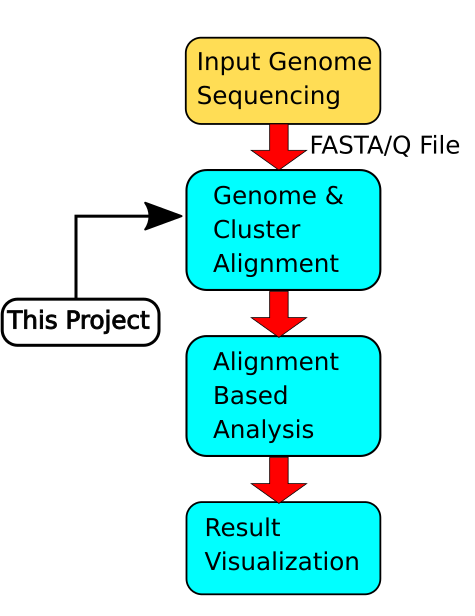
\includegraphics[scale = 0.4]{Figures/pipeline.png}
    \caption{Sera remplacé par une figure de la pipeline}
    \label{fig:analysispipe}
\end{figure}
\end{minipage}
\begin{minipage}[t]{0.350\textwidth}
After being read, usual genome sequencer produce 5 types of symbols, the 4 nucleobases A, C, G, T and another symbol, $N$, present when the sequencer could not determine which base to assign to a read sample. Then comes the alignment, an essential step to any further work on those data. [......] \\

\end{minipage}
\vspace*{5mm}



As an obligatory procedure to any further work on genomic data, increasing the performance on read alignment seems greatly needed. As mentioned earlier, processing those pieces of information means processing a huge volume of rather redundant textual data. This distinctive aspect makes room already for a lot of optimization including data compression and parallel processing and this is where another approach might be pertinent. \\

Hardware accelerators are now a common practice\footnote{CITE} when confronted to a need of performance gain for a specific task in an information system. This approach seems indeed to be very efficient by providing a fully dedicated highly parallelizable system, meaning very little to no processing overhead, for those tasks. In this context, the sequence mapping of a plethora of short reads to one common reference seems like an ideal candidate for such an approach. This idea is the main scope of this project and will be further detailed in the next section.

\section{Research Question}

As mentioned in the previous section beyond the urgent need of quick performance improvement of short read alignment in genomic data processing, there might be a real speedup potential in the use of a hardware accelerator for this part of the analysis pipeline. 

With this in mind, this project will try to propose an hardware implementation of the FM-Index. The main idea is to provide a time and memory efficient solution as an alternative to otherwise entirely software solutions. In a second phase, this project will try to explore the performances of such a model in order to determine a final solution offering a significant speedup.

\section{Method Introduction}

This project will start with a custom software implementation of the FM-Index, in \textsl{C++}, in order to both get a better grasp of the concepts at stake, and provide a communication interface for the future hardware module.

 For this second phase, among many hardware solutions, \textsl{FPGAs} seem like an ideal candidate. Enabling a fully dedicated hardware design and able to use  highly efficient data [management ??] tools (pour dire mémoire et bus).

Using \textsl{Hybrid Memory Cube} to store the reference data and \textsl{PCI Express} bus to communicate with a computer, both of which will be further introduced in an upcoming section, this project will then try to design a simple and low latency FM-Index implementation in \textsl{VHDL}. Then, in a final phase, it will try to explore the parallelization possibilities of this solution in order to make the best out of both \textsl{FPGA} and \textsl{HMC} provided advantages.